\documentclass{beamer}

\usepackage{beamerthemesplit}
\usepackage{pgf}

\usetheme{Berkeley}
\useinnertheme{circles}
\usecolortheme{seagull}

\title[Stereo vision]{Stereo Vision using the OpenCV library \\ A glance}
\author[Dr\"oppelmann \and Hueting \and Latour \and \\Van der Veen]{Sebastian Dr\"oppelmann \\ Moos Hueting \\ Sander Latour \\ Martijn van der Veen}
\institute{University of Amsterdam}
\date{June 2010}
\subject{Computer vision}

\begin{document}

\graphicspath{{./images/}}

\frame
{
  \titlepage
}

\section{Recap}

\frame
{
 \frametitle{Goal}
 \begin{block}{Goal}
   Generating a disparity depth map of the environment using stereo vision.
 \end{block}
}

\frame{
 \frametitle{Intended end-result}
 \begin{figure}
   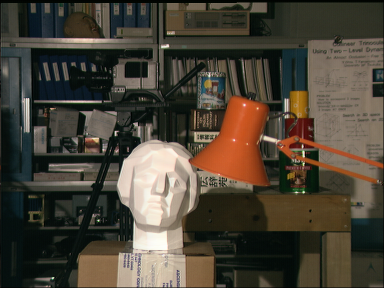
\includegraphics[width=0.3\textwidth]{exampleleft}
   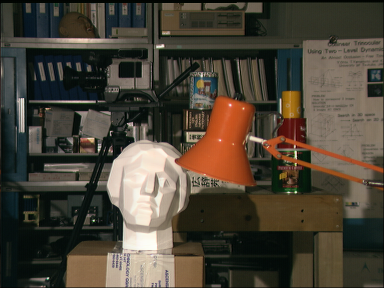
\includegraphics[width=0.3\textwidth]{exampleright}
   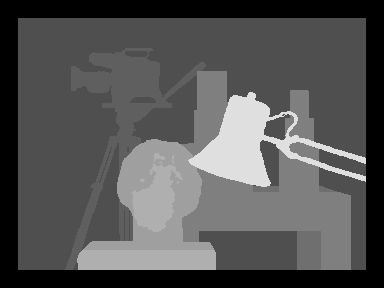
\includegraphics[width=0.3\textwidth]{exampledepth}
   \caption{Stereo images with disparity depth map}
 \end{figure}
}

\section{Demonstration}

\frame{
  \frametitle{Calibration}
  \begin{itemize}
    \item Retrieve distortion
    \item Retrieve spatial relation between cameras
  \begin{figure}[h!]
    \centering
    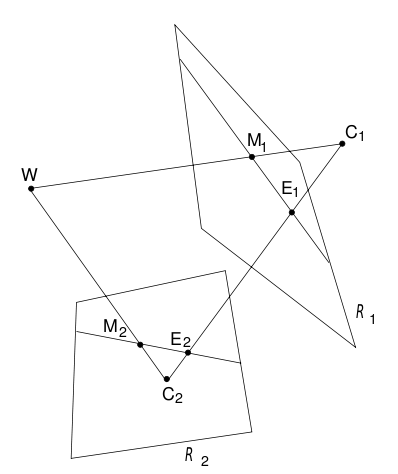
\includegraphics[width=0.4\textwidth]{nonrectepipole.png}
    %\caption{Non-rectified camera's}
  \end{figure}
  \end{itemize}
}

\frame{
  \frametitle{Calibration}
  Demo
}

\frame{
  \frametitle{Epipolar Geometry}

  \begin{figure}[h!]
    \centering
    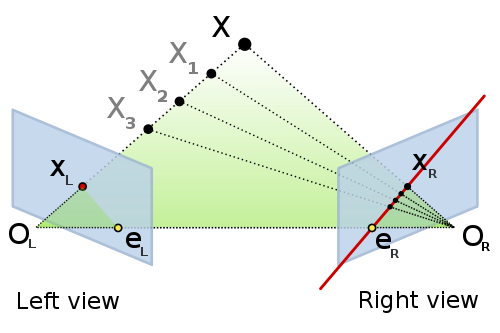
\includegraphics[width=0.5\textwidth]{500px-Epipolar_geometry.png}
    \caption{Epipolar geometry. Point $X_L$ in the left image has to lie on the epipolar line in the right image}
  \end{figure}

}

\frame{
  \frametitle{Rectification}
  \begin{itemize}
    \item Calculate rectification parameters
    \item Reusable
  \begin{figure}[h!]
    \centering
    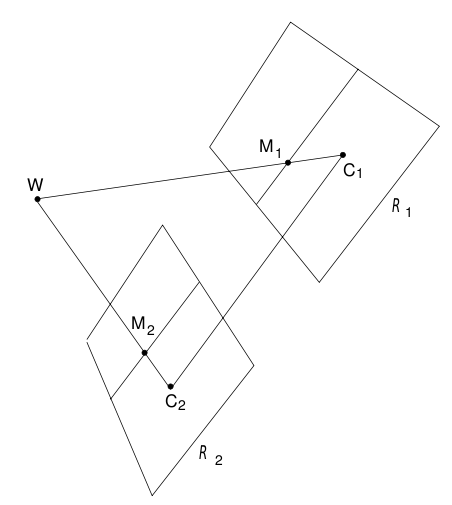
\includegraphics[width=0.4\textwidth]{rectepipole.png}
    %\caption{Rectified camera's}
  \end{figure}
  \end{itemize}
}

\frame{
  \frametitle{Rectification}
   Demo
}

\frame{
  \frametitle{Stereo Matching - A general overview}
  % PGF Latex Image
% Shows two images with pixels {A,B,C,D,E,F,G,H} with disparity and occlusion.
\begin{pgfpicture}
\color{black}
\pgfrect[stroke]{\pgfxy(0,1.5)}{\pgfxy(.5,.5)}
\pgfrect[stroke]{\pgfxy(.5,1.5)}{\pgfxy(.5,.5)}
\pgfrect[stroke]{\pgfxy(1,1.5)}{\pgfxy(.5,.5)}
\pgfrect[stroke]{\pgfxy(0,2)}{\pgfxy(.5,.5)}
\pgfrect[stroke]{\pgfxy(.5,2)}{\pgfxy(.5,.5)}
\pgfrect[stroke]{\pgfxy(1,2)}{\pgfxy(.5,.5)}
\pgfrect[stroke]{\pgfxy(0,2.5)}{\pgfxy(.5,.5)}
\pgfrect[stroke]{\pgfxy(.5,2.5)}{\pgfxy(.5,.5)}
\pgfrect[stroke]{\pgfxy(1,2.5)}{\pgfxy(.5,.5)}
\pgfputat{\pgfxy(0.25,1.75)}{\pgfbox[center,center]{G}}
\pgfputat{\pgfxy(0.75,1.75)}{\pgfbox[center,center]{H}}
\pgfputat{\pgfxy(1.25,1.75)}{\pgfbox[center,center]{I}}
\pgfputat{\pgfxy(0.25,2.25)}{\pgfbox[center,center]{D}}
\pgfputat{\pgfxy(0.75,2.25)}{\pgfbox[center,center]{E}}
\pgfputat{\pgfxy(1.25,2.25)}{\pgfbox[center,center]{F}}
\pgfputat{\pgfxy(0.25,2.75)}{\pgfbox[center,center]{A}}
\pgfputat{\pgfxy(0.75,2.75)}{\pgfbox[center,center]{B}}
\pgfputat{\pgfxy(1.25,2.75)}{\pgfbox[center,center]{C}}

\pgfrect[fill]{\pgfxy(2,1.5)}{\pgfxy(.5,.5)}
\pgfrect[fill]{\pgfxy(2.5,1.5)}{\pgfxy(.5,.5)}
\pgfrect[stroke]{\pgfxy(3,1.5)}{\pgfxy(.5,.5)}
\pgfrect[fill]{\pgfxy(2,2)}{\pgfxy(.5,.5)}
\pgfrect[fill]{\pgfxy(2.5,2)}{\pgfxy(.5,.5)}
\pgfrect[stroke]{\pgfxy(3,2)}{\pgfxy(.5,.5)}
\pgfrect[fill]{\pgfxy(2,2.5)}{\pgfxy(.5,.5)}
\pgfrect[stroke]{\pgfxy(2.5,2.5)}{\pgfxy(.5,.5)}
\pgfrect[stroke]{\pgfxy(3,2.5)}{\pgfxy(.5,.5)}

\pgfputat{\pgfxy(3.25,1.75)}{\pgfbox[center,center]{H'}}
\pgfputat{\pgfxy(3.25,2.25)}{\pgfbox[center,center]{D'}}
\pgfputat{\pgfxy(2.75,2.75)}{\pgfbox[center,center]{A'}}
\pgfputat{\pgfxy(3.25,2.75)}{\pgfbox[center,center]{B'}}

\pgfputat{\pgfxy(1.75,2.25)}{\pgfbox[center,center]{$\Rightarrow$}}
\end{pgfpicture}
  \begin{itemize}
   \item Mapping of pixels
   \item Disparity $\rightarrow$ Depth
   \item Occlusion
  \end{itemize}
}

\frame{
  \frametitle{Stereo Matching - Depthmap}
  \begin{figure} [h!tb]
  \centering
  \begin{minipage}[h]{.4\linewidth}
  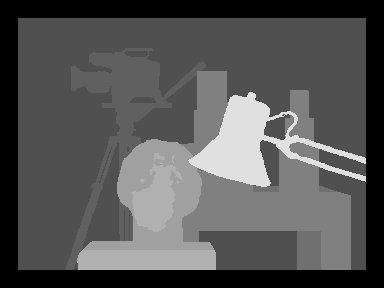
\includegraphics[width=\textwidth]{disp_tsukuba_orig}
  \end{minipage}
  \hspace{.1\linewidth}
  \begin{minipage}[h]{.4\linewidth}
  % PGF Latex Image
% Shows two images with pixels {A,B,C,D,E,F,G,H} with disparity and occlusion.
\definecolor{light-gray}{gray}{0.75}
\definecolor{dark-gray}{gray}{0.35}
\begin{pgfpicture}

\color{black}
\pgfrect[fill]{\pgfxy(0,0)}{\pgfxy(.5,.5)}
\color{dark-gray}
\pgfrect[fill]{\pgfxy(0,.5)}{\pgfxy(.5,.5)}
\color{gray}
\pgfrect[fill]{\pgfxy(0,1)}{\pgfxy(.5,.5)}
\color{light-gray}
\pgfrect[fill]{\pgfxy(0,1.5)}{\pgfxy(.5,.5)}
\color{black}
\pgfrect[stroke]{\pgfxy(0,2)}{\pgfxy(.5,.5)}
\pgfrect[stroke]{\pgfxy(0,1.5)}{\pgfxy(.5,.5)}
\pgfrect[stroke]{\pgfxy(0,1)}{\pgfxy(.5,.5)}
\pgfrect[stroke]{\pgfxy(0,.5)}{\pgfxy(.5,.5)}
\pgfrect[stroke]{\pgfxy(0,0)}{\pgfxy(.5,.5)}
\pgfputat{\pgfxy(1.2,0.2)}{\pgfbox[center,center]{Invalid}}
\pgfputat{\pgfxy(1.35,0.73)}{\pgfbox[center,center]{Very Far}}
\pgfputat{\pgfxy(0.90,1.25)}{\pgfbox[center,center]{Far}}
\pgfputat{\pgfxy(1.2,1.70)}{\pgfbox[center,center]{Nearby}}
\pgfputat{\pgfxy(1.2,2.25)}{\pgfbox[center,center]{Closest}}
\end{pgfpicture}
  \end{minipage}
  \end{figure}
}


\frame {
  \frametitle{Stereo Algorithms - Graph Cut}
      \begin{itemize}
      \item popular
      \item slow
      \item smooth
      \item interlinear consistency
      \end{itemize}
      \begin{figure}
      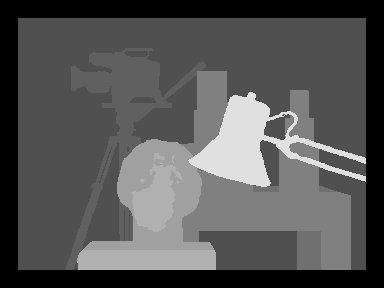
\includegraphics[width=0.4\textwidth]{disp_tsukuba_orig}
      \:
      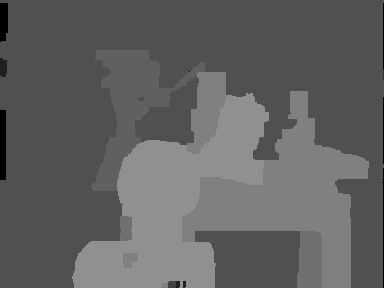
\includegraphics[width=0.4\textwidth]{gc_tsukuba_own}
      \end{figure}
}


\frame {
  \frametitle{Stereo Algorithms - Block Matching}
    \begin{itemize}
      \item fast
      \item lots of noise
    \end{itemize}
    \begin{figure}
    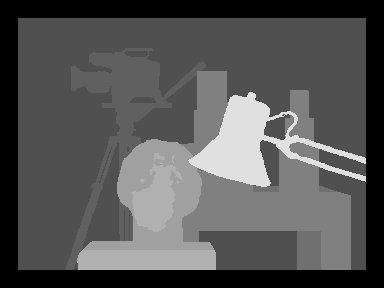
\includegraphics[width=0.4\textwidth]{disp_tsukuba_orig}
    \:
    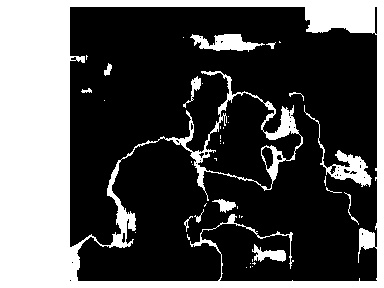
\includegraphics[width=0.4\textwidth]{bm_tsukuba_own}
    \end{figure}

}

\frame{
    \frametitle{Stereo Algorithms - Semi Global Block Matching}
    \begin{itemize}
      \item not in Python
      \item good in speed/quality
      \item good depthmap
      \item noise
    \end{itemize}
    \begin{figure}
    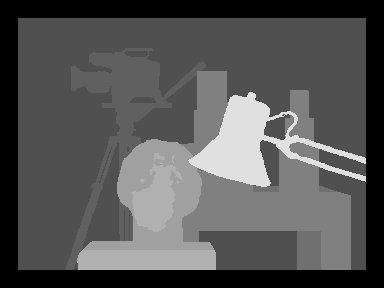
\includegraphics[width=0.4\textwidth]{disp_tsukuba_orig}
    \:
    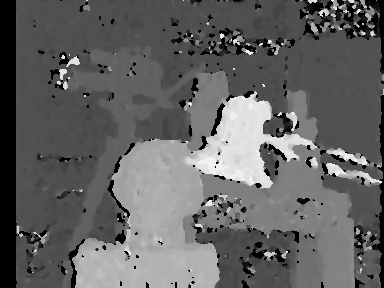
\includegraphics[width=0.4\textwidth]{sgbm_tsukuba_own}
    \end{figure}
}

\section{Applications}

\frame{
  \frametitle{Demo}
  \begin{itemize}
   \item 3D mapping of a 2D image
   \item Live Depthmap
   \item Background Removal
  \end{itemize}
}

\section{Vragen}
\frame{
  \frametitle{Vragen?}
}

\end{document}
